\documentclass[12pt]{article}
\usepackage{a4,fancyhdr,moreverb,epsfig,amssymb,amsmath,amsthm,ifthen,listings, graphicx, fancyvrb}
\usepackage[usenames,dvipsnames]{color}
\usepackage[makeroom]{cancel}

\textwidth 455pt \oddsidemargin 0mm
\parindent 0pt
\textheight 685pt % old : 665pt
\textheight 697pt
\topmargin -40pt  % old -70pt
\renewcommand{\vec}{\underline}
\newcommand{\va}{\underline{a}}
\newcommand{\vb}{\underline{b}}
\newcommand{\vc}{\underline{c}}
\newcommand{\vh}{\underline{h}}
\newcommand{\ve}{\underline{e}}
\newcommand{\vg}{\underline{g}}
\newcommand{\vp}{\underline{p}}
\newcommand{\vq}{\underline{q}}
\newcommand{\vu}{\underline{u}}
\newcommand{\vv}{\underline{v}}
\newcommand{\vw}{\underline{w}}
\newcommand{\vx}{\underline{x}}
\newcommand{\vy}{\underline{y}}
\newcommand{\vz}{\underline{z}}
\newcommand{\dx}{\; {\rm d}x}
\newcommand{\dbydx}[1]{\frac{d}{dx}\left( #1 \right)}
\newcommand{\dfdx}{\frac{{\rm d}f}{{\rm d}x}}
\newcommand{\dfstardx}{\frac{{\rm d}f_n^*}{{\rm d}x}}
\newcommand{\dfpstardx}{\frac{{\rm d}f_p^*}{{\rm d}x}}
\newcommand{\ddx}[2]{\frac{{\rm d}^#1#2}{{\rm d}x^#1}}
\newcommand{\inprod}[2]{\langle #1, #2 \rangle}
\newcommand{\sinmpiddot}{\sin \left(\frac{m\,\pi\,\cdot}{d}\right)}
\newcommand{\sinmpid}{\sin \left(\frac{m\,\pi}{d}\right)}
\newcommand{\cosmpixd}{\cos \left(\frac{m\,\pi\,x}{d}\right)}
\newcommand{\sinmpixd}{\sin \left(\frac{m\,\pi\,x}{d}\right)}
\newcommand{\cosmpid}{\cos \left(\frac{m\,\pi}{d}\right)}
\newcommand{\cosmpiddot}{\cos \left(\frac{m\,\pi\,\cdot}{d}\right)}
\newcommand{\norm}[1]{\left\|#1\right\|}
\newcommand{\intd}{\int_{-d}^d}
\newcommand{\integ}[1]{\int_{-#1}^#1}
\newcommand{\intzero}[1]{\int_{0}^#1}

\lstset{language=Python,
                basicstyle=\small,
                keywordstyle=\color{blue}\ttfamily,
                morekeywords={bool},
                stringstyle=\color{red}\ttfamily,
                commentstyle=\color{Plum}\ttfamily,
	      showstringspaces=false,
                morecomment=[l][\color{BurntOrange}]{\#}
}

\begin{document}
\pagestyle{fancyplain}
\lhead{\fancyplain{}{\sf M2AA3, Introduction to Numerical Analysis}}
\rhead{\fancyplain{}{\sf Jaime Rodriguez. CID 870873}}
\cfoot{}{}


\begin{center} \Large
M2AA3 -- Project 2 \\[4mm]
\end{center}





\section{Formal proofs}
\subsection{A}


First, given that $\dfdx \in V$ and $f(-d)=f(d)$, let's show that
\begin{align*}
&\langle \dfdx (\cdot),
\sin \left(\frac{m\,\pi\,\cdot}{d}\right)\rangle
= - m\,\pi\,a_m,
\qquad
\langle \dfdx (\cdot),
\cos \left(\frac{m\,\pi\,\cdot}{d}\right)\rangle
= m\,\pi\,b_m, 
\qquad m=1 \rightarrow n\,;
\end{align*}

Let's compute $\inprod{\dfdx (\cdot)}{\sinmpiddot}$. By our definition of the inner product, \\\\

\begin{equation}
\begin{aligned}
\inprod{\dfdx(\cdot)}{\sinmpiddot} &= \intd \dfdx(x) \sinmpixd dx\\
	&= \left[\sinmpixd f(x)\right]_{-d}^d - \frac{m \pi}{d} \intd f(x)  \cosmpixd dx\\
	%\intertext{Using the definition of $a_m$, we get that}
	&= \sin \left(m\,\pi\right)\,f(d) - \sin \left(-m\,\pi\right)\,f(-d) - m\,\pi\,\frac{1}{d}\,\inprod{f(\cdot)}{\cosmpiddot}\\
	%\intertext{Since $\sin \left(m \pi\right) = 0$, for all $m \in \mathbb{Z}$}
	&= - m\,\pi\,\frac{1}{d}\,\inprod{f(\cdot)}{\cosmpiddot}\\
	&= -m\,\pi\,a_m
\end{aligned}
\end{equation}


Similarly for $\inprod{\dfdx (\cdot)}{\sinmpiddot}$,
\begin{equation}
\begin{aligned}
\inprod{\dfdx(\cdot)}{\cosmpiddot} &= \intd \dfdx(x) \cosmpixd dx\\
	&= \left[\cosmpixd f(x)\right]_{-d}^d - \frac{m \pi}{d} \intd f(x)  \sinmpixd dx\\
	&=  m\,\pi\,\frac{1}{d}\,\inprod{f(\cdot)}{\sinmpiddot}\\
	&= m\,\pi\,b_m 
\end{aligned}
\end{equation}
\subsection{B}
From here we must conclude that,
\begin{align*}
\left\|\dfdx -\dfstardx\right\| &\leq 
\left\|\dfdx -v_n\right\| \qquad \forall\ v_n \in V_n
\end{align*}
In other words, we must prove that the best the best approximation to $\dfdx$ in $\|\cdot\|$ from $V_n$ is $\dfstardx$.

Let the best approximation to $\dfdx$  in $\|\cdot\|$ from $V_n$ be $v^*$.
From our results in lectures, we know that this is true if and only 
\begin{equation}
\begin{aligned}
	v^{*} &= \frac{\inprod{\dfdx}{1}}{\norm{1}^2}\cdot\,1 + 
			\sum_{m = 1}^n \frac{\inprod{\dfdx}{\cosmpixd}}{\norm{\cosmpixd}^2}\,\cosmpixd +
			\sum_{m = 1}^n \frac{\inprod{\dfdx}{\sinmpixd}}{\norm{\sinmpixd}^2}\,\sinmpixd\\
	&= \frac{1}{d} \left( \frac{1}{2}\underbrace{\intd{\dfdx dx}}_{f(d) - f(-d)\, =\, 0} +
						  \pi\,\sum_{m = 1}^n m\,b_m \, \cosmpixd - 
						  \pi\,\sum_{m = 1}^n m\,a_m \, \sinmpixd 
				   \right)\\
	&= \sum_{m = 1}^n \left(  \frac{\pi\,m}{d}\,b_m \, \cosmpixd - \frac{\pi\,m}{d}\,a_m \, \sinmpixd \right)
\end{aligned}
\end{equation}
Where we have used the fact that  $\norm{\cosmpixd}^2$ and $\norm{\sinmpixd}^2$ take the value d.\\

We can see that $v^*$ is in the form of a Fourier series with coefficients
\begin{align}
	a_0' = 0, \qquad\,
	a_m' =  \frac{\pi\,m}{d}\,b_m, \qquad\,
	b_m' = - \frac{\pi\,m}{d}\,a_m, \qquad\,
	m = 1\,...\,n
\end{align}

To prove that $v^* = \dfstardx$, we must check that differentiating the expression for $\dfdx$
creates an expression with identical coefficients. By definition,
\begin{align}
f_n^\star(x) 
= \frac{a_0}{2} + \sum_{m=1}^n \left[ a_m \,\cos \left(\frac{m\,\pi\,x}{d}
\right) + b_m\,\sin \left(\frac{m\,\pi\,x}{d}\right)\right] ,
\end{align}

Differentiating this expression with respect to x, $a_0$ differentiates to 0 because it is a constant, the rest is as follows,
\begin{align}
\dfstardx(x) 
	&= 0 + \sum_{m=1}^n \left[ a_m \,\dbydx{\cos \left(\frac{m\,\pi\,x}{d} \right)} +
				b_m\,\dbydx{\sin \left(\frac{m\,\pi\,x}{d}\right)}\right]
	\\ &= \sum_{m=1}^n \left[ \underbrace{\frac{\pi\,m}{d}\,b_m}_{a_m'}\,\cos \left(\frac{m\,\pi\,x}{d}\right) -
						\underbrace{\frac{\pi\,m}{d}\,a_m}_{b_m'} \,sin \left(\frac{m\,\pi\,x}{d} \right) \right]
\end{align}
We can see that the coefficients of $\dfstardx$ are the same as the ones for $v^*$. Therefore, we conclude
that $\dfstardx = v^*$ and hence our best approximation to $\dfdx$ in $\|\cdot\|$ from $V_n$ is $\dfstardx$
for all functions $f \in V$.

\subsection{C}
Now, we are given that the best approximation to $\dfdx$ in $\|\cdot\|$ from $V_n$ is such that
\begin{align*}
\norm{\dfdx-\dfstardx} &\leq \norm{\dfdx-v_n} \qquad \forall \ v_n \in V_n \\
\mbox{and} \qquad  d\,\left(\frac{a_0'^2}{2} + \sum_{m=1}^n [a_m'^2 + b_m'^2]
\right)
& = \norm{\dfstardx}^2 = \norm{\dfdx}^2 - \norm{\dfdx-\dfstardx}^2. 
\end{align*}

Plugging in the coefficients $a_0'$, $a_m'$ and $b_m'$ for m = $1\,...\,n$ computed earlier,

\begin{align}
	d\,\left(\frac{a_0'^2}{2} + \sum_{m=1}^n [a_m'^2 + b_m'^2] \right) &=
	d\,\left(0 + \sum_{m=1}^n [\left(\frac{\pi\,m}{d}b_m\right)^2 +
							   \left(- \frac{\pi\,m}{d}\,a_m\right)^2]\right)\\
	&= \frac{\pi^2}{d} \sum_{m=1}^n m^2 (a_m^2 + b_m^2)\\
	&= \norm{\dfstardx}^2\\
	&= \norm{\dfdx}^2 - \norm{\dfdx-\dfstardx}^2\\
	&\leq \norm{\dfdx}^2
\end{align}
The last step following because  $\norm{\dfdx-\dfstardx}^2$ is always positive, as it is the square of
the norm.
\subsection{D}

Hence show that
\begin{align*}
\lim_{m \to \infty} m\,a_m  = \lim_{m \to \infty} m\,b_m =0\,.   
\end{align*}

The previous result gives us that $\frac{\pi^2}{d} \sum_{m=1}^n m^2 (a_m^2 + b_m^2)$ is positive and bounded above by a finite value $\norm{\dfdx}^2$.

Rearranging this gives us the series,
\begin{align}
	0 \leq \sum_{m=1}^n (m\,a_m)^2 + (m\,b_m)^2 \leq K
\end{align}
for some constant K (which we know is finite).

From M1PM1, we know that a series where every term is non-negative converges if and only if it is bounded. Hence we get that our series converges. This necessarily implies that the sequence of terms tends to 0.

Finally, since both terms $(m\,a_m)^2$ and $(m\,b_m)^2$ are positive, we see that they both must tend to zero as $m \rightarrow \infty$.

Hence, 

$\lim_{m \to \infty} m\,a_m  = \lim_{m \to \infty} m\,b_m =0\,.  $\\

\subsection{E}

Now for $d=1$ and $f(x)=x^2$, 
find the coefficients $\{a_m\}_{m=0}^n$ and $\{b_m\}_{m=1}^n$
in $f_n^\star$ and find expressions for $\| f - f_n^* \|^2$
and $\left\| \dfdx - \dfstardx \right\|^2$.\\
First compute $a_0$,
\begin{align}
	a_0 &= \frac{1}{d}\inprod{x^2}{1}\\
		&= \integ{1} x^2 \dx = \left[\frac{x^3}{3}\right]_{-1}^{1} = \frac{2}{3} 
\end{align}
Now $a_m$,
\begin{align}
	a_m &= \frac{1}{d}\inprod{x^2}{\cos(m\pi\,x)}\\
		&= \frac{1}{1} \integ{1} x^2\,\cos(m\,\pi\,x) \dx\\
	 	\intertext{Since the product of even functions is an even function, the integral doubles over a symmetric range, and hence,}
	 	&= 2 \intzero{1} x^2\,\cos(m\,\pi\,x) \dx\\
	 	\intertext{Then integrating by parts}
	 	&= 2 \left(\underbrace{\left[\frac{x^2\,sin(m\pi\,x)}{m\,\pi}\right]_0^1}_{\text{This is 0}} -
	 					 \frac{2}{m\pi} \intzero{1} x\,sin(m\pi\,x) \dx\right)\\
	 	\intertext{And integrating the second integral by parts again}
	 	&= -\frac{4}{m\pi} \left(\left[\frac{-x\,\cos(m\pi\,x)}{m\,\pi}\right]_0^1 +
	 					 \frac{1}{\pi\,m} \intzero{1} \cos(m\pi\,x) \dx\right)\\
	 	&= -\frac{4}{m\pi} \left(\frac{(-(-1)^m - 0)}{m\pi} +
	 					 \left(\frac{1}{\pi\,m}\right)^2 \underbrace{\cancel{\left[sin(m\pi\,x)\right]_0^1}}_{0}\right)\\
	 	&= \frac{4}{m^2\pi^2} (-1)^m = a_m\, \tag{For m = 1...n}
\end{align}

However, $b_m$ is much easier to compute. Given that $x^2$ is an even function and $sin(m\pi\,x)$ is odd,
we know that over a symmetric domain the integral collapses to zero. Thus
\begin{align}
		b_m &= \frac{1}{1}\inprod{x^2}{sin(m\pi\,x)}\\
			&= \underbrace{\integ{1} x^2\,sin(m\,\pi\,x) \dx}_{\text{Odd function}}
			= 0 \tag{For m = 1...n}
\end{align}

Giving us the Fourier Series for $f_n^*$:
\begin{align}
	f_n^*(x) = \frac{2}{3} + \frac{4}{\pi^2}\sum_{m=1}^n
			\frac{(-1)^m}{m^2} \cos(m\,\pi\,x)
\end{align}
Now we can find an expression for $\norm{f - f_n^*}^2$. Using the expression
\begin{align}
	\|f_n^\star\|^2 = \|f\|^2 - \|f-f_n^\star\|^2
\end{align}
we can rearrange to get
\begin{align}
	\|f-f_n^\star\|^2 = \|f\|^2 - \|f_n^\star\|^2 
\end{align}

Let's find expressions for the two norms on the right hand side of the inequality.
First,
\begin{align}
	\norm{f}^2 = \inprod{f}{f} = 2 \intzero{1} x^4 \dx = \frac{2}{5}
\end{align}
Then, for the second term, we know that
\begin{align}
	\norm{f_n^*}^2 = d\left(\frac{a_0^2}{2} + \sum_{m=1}^n [a_m^2 + b_m^2]\right)
\end{align}
Thus plugging in the coefficients we found,
\begin{align}
		\norm{f_n^*}^2 = \frac{2}{9} + \frac{16}{\pi^2}\sum_{m=1}^n \frac{1}{m^4}
\end{align}

This leads to the expression we were searching for,
\begin{align}
	\|f-f_n^\star\|^2 = \|f\|^2 - \|f_n^\star\|^2 = \frac{8}{45} - \frac{16}{\pi^4} \sum_{m=1}^n \frac{1}{m^4}
\end{align}

Now to find $\left\| \dfdx - \dfstardx \right\|^2$, we must compute the coefficients $a_0'$, $a_m'$ and $b_m'$ of $\dfstardx$ for $m = 1...n$.

Now our function $\dfdx$ is $\dfdx = 2x$, an odd function. Hence, we quickly see that $a_m' = 0$ for $m = 0...n$, since the integrals will collapse when we combine $2x$ with the cosine terms (or 1 in case of $a_0$), as they will be odd fuctions over a symmetric interval.

Let's compute $b_m$ for $m = 1...n$,

\begin{align}
	b_m' &= \frac{1}{d}\inprod{2x}{sin(m\pi\,x)}\\
		&= \frac{1}{1} \integ{1} 2x\,sin(m\,\pi\,x) \dx\\
	 	\intertext{Doubling the integral of an even function over a symmetric range,}
	 	&= 4 \intzero{1} x\,sin(m\,\pi\,x) \dx\\
	 	\intertext{Then integrating by parts}
	 	&= 4 \left(\left[\frac{-x\,\cos(m\pi\,x)}{m\,\pi}\right]_0^1 +
	 					 \frac{1}{m\pi} \intzero{1} \cos(m\pi\,x) \dx\right)\\
	 	&= 4 \left(-\frac{1}{m\pi}(-1)^m + \frac{1}{m\pi}\underbrace{\cancel{\left[\frac{sin(m\pi\,x)}{m\pi}\right]_0^1}}_{0}\right)\\
	 	&= -\frac{4}{m\pi} (-1)^m \tag{For m = 1...n}
\end{align}


Leading to the Fourier Series of $\dfdx = 2x$, 
\begin{align}
	\dfstardx (x) = \frac{-4}{\pi}\sum_{m=1}^n
			\frac{(-1)^m}{m} sin(m\,\pi\,x) 
\end{align}
It follows that
\begin{align}
	\norm{\dfstardx}^2 &= d\left(\frac{a_0'^2}{2} + \sum_{m=1}^n [a_m'^2 + b_m'^2\right)\\
		&= \frac{16}{\pi^2}\sum_{m=1}^n \frac{1}{m^2}
\end{align}

Also,
\begin{align}
	\norm{\dfdx}^2 = \integ{1} (2x)^2 = 4 \left[\frac{x^3}{3}\right]_{-1}^1 =  \frac{8}{3}
\end{align}

And finally,
\begin{align}
	\left\| \dfdx - \dfstardx \right\|^2 = \frac{8}{3} - \frac{16}{\pi^2}\sum_{m=1}^n \frac{1}{m^2}
\end{align}
\subsection{F}
Next, we need to show, using trigonometric identities, that for $n \geq 1$
\begin{alignat*}{2}
\ddx{2}{[f-f_{n}^*]}(x) & =\frac{2\,(-1)^n\,\cos((n+\frac{1}{2})\,\pi\,x)}
{\cos(\frac{\pi\,x}{2})} \qquad && x \in (-1,1) \,,\\
\text{and hence }\ \qquad \ddx{2}{[f-f_{n}^*]} (\pm \textstyle
\frac{2\,k-1}{2\,n+1}) & =0 \quad && k=1 \rightarrow n.
\end{alignat*}
Let's prove the first part.


\begin{equation}
	\begin{aligned}
		\ddx{2}{[f-f_{n}^*]}(x) &= \dbydx{\dfdx - \dfstardx} = \frac{d^2\,f}{\dx} - \dbydx{\dfstardx}\\
		&= 2 - \dbydx{\frac{-4}{\pi}\sum_{m=1}^n
			\frac{(-1)^m}{m} \sin(m\,\pi\,x)  }\\
		&= 2 + \frac{4}{\pi}\sum_{m=1}^n
			\frac{(-1)^m}{m} \dbydx{\sin(m\,\pi\,x)}\\
		&= 2 + 4\sum_{m=1}^n
			(-1)^m\, \cos(m\,\pi\,x)
	\end{aligned}
\end{equation}
For the next few steps, I will use the following trigonometric identity.
\begin{align}
	\cos(a) \cdot \cos(b) = \frac{1}{2} \left(\cos(a + b) + \cos(a - b) \right)
\end{align}

Let's focus on the summation.
\begin{equation}
	\begin{aligned}
		2 * \sum_{m=1}^n (-1)^m\, \cos(m\,\pi\,x)
			&= \frac{2}{\cos(\frac{\pi}{2}x)}\sum_{m=1}^n (-1)^m\, \cos(m\,\pi\,x)\, \cos(\frac{\pi}{2}x)\\
		&= \frac{\sum_{m=1}^n (-1)^m\, \left(\cos((m+\frac{1}{2})\,\pi\,x) +
						\cos((m-\frac{1}{2})\,\pi\,x)\right)}{\cos(\frac{\pi}{2}x)}\\
	\end{aligned}
\end{equation}
Now notice how the inner terms of the summation cancel out.
\begin{align}
	-(\cancel{\cos(\frac{3}{2}\,\pi\,x)} +  \cos(\frac{1}{2}\,\pi\,x))
	+ (\cancel{\cos(\frac{5}{2}\,\pi\,x)} + \cancel{\cos(\frac{3}{2}\,\pi\,x)})
	- \cdots\\
	+ (-1)^n(\cos((n + \frac{1}{2})\,\pi\,x) + \cancel{\cos(n - \frac{1}{2})\,\pi\,x)}
\end{align}
And we are left with the following.
\begin{equation}
	\begin{aligned}
		\ddx{2}{[f-f_{n}^*]}(x) &= 2 + 2 * \frac{-\cos(\frac{\pi}{2}\,x) + 
			(-1)^n \cos((n + \frac{1}{2})\,\pi\,x))}{\cos(\frac{\pi}{2}x)}\\
			&= \frac{2(-1)^n\,\cos((n+\frac{1}{2})\,\pi\,x)}{\cos(\frac{\pi}{2}\,\pi\,x)}\\
	\end{aligned}
\end{equation}\\
 

The second part follows easily. We can plug in $x = \frac{2k-1}{2n+1}$ into the derived form, since
$\frac{2k-1}{2n+1} \in (-1, 1)$ due to the fact that $k = 1 \rightarrow n$ implies $k \leq n$.
\begin{align}
	\ddx{2}{[f-f_{n}^*]}\left(\frac{2k-1}{2n+1}\right)
		& =\frac{2\,(-1)^n\,\cos((n+\frac{1}{2})\,\pi\,\left(\frac{2k-1}{2n+1}\right))} {\cos(\frac{\pi}{2}\frac{2k-1}{2n+1})}\\
		&= \frac{2\,(-1)^n\,\cos((\frac{2n+1}{2})\,\pi\,\left(\frac{2k-1}{2n+1}\right))} {\cos(\frac{\pi}{2}\frac{2k-1}{2n+1})}\\
		& =\frac{2\,(-1)^n\,\cos(\frac{\pi}{2}(2k-1))} {\cos(\frac{\pi}{2}\frac{2k-1}{2n+1})}
		= 0
\end{align}
The last equality holding thanks to $\cos(t \pi) = 0$ for t an odd number.

\section{Computer calculations in Python}

The first piece of code computes $\norm{f - f_n^*}^2$ and then plots $f(x)$ and $f_n^*$ for $x \in (-1, 1)$ for $n = 1 \rightarrow 9$.\\
\lstinputlisting{fourier.py}

\textbf{This is the output it generated}
\verbatiminput{output1.txt}
\clearpage
\textbf{PLOTS}\\

\hspace{-3em}
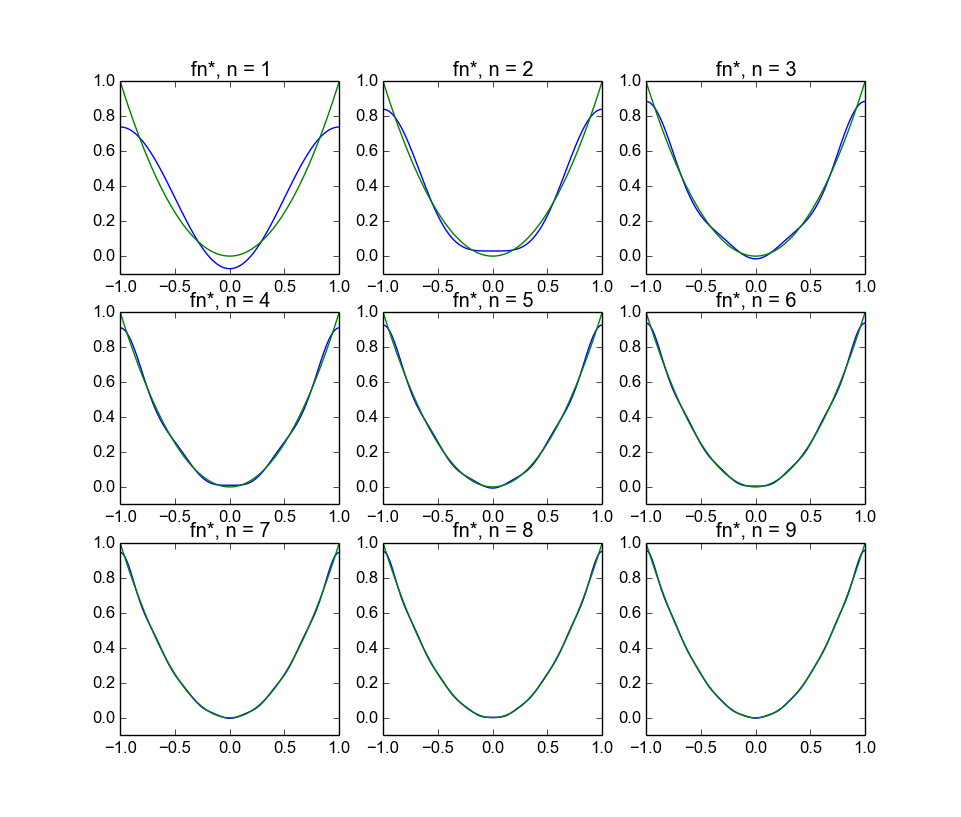
\includegraphics[scale=0.75]{graphsf.png}
%\clearpage

The next piece is very similar to the previous section. It computes $\norm{\dfdx - \dfstardx}^2$ and then plots $\dfdx(x)$ and $\dfstardx^*$ for $x \in (-1, 1)$ for $n = 1 \rightarrow 9$. I only include the differences with respect to the previous code.\\

\begin{lstlisting}
# Function df/dx
df = lambda x : 2 * x

# Fourier series approximation to df/dx with n terms
def df_best_approx(x, n):
    val = 0.0
    for m in range(1, n + 1):
        val += ((-1) ** m) * math.sin(m * math.pi * x) / m
    val *= (-4) / math.pi
    return val

# Formula derived for ||f-fn*||^2
def difference_formula(n):
    res = float(8) / 3 
    val = 0.0
    for m in range(1, n + 1):
        val -= float(1) / (m ** 2)
    val *= 16 / (math.pi ** 2)
    return res + val
\end{lstlisting}

\textbf{This is the output it generated}
\verbatiminput{output2.txt}
\clearpage
\textbf{PLOTS}\\

\hspace{-3em}
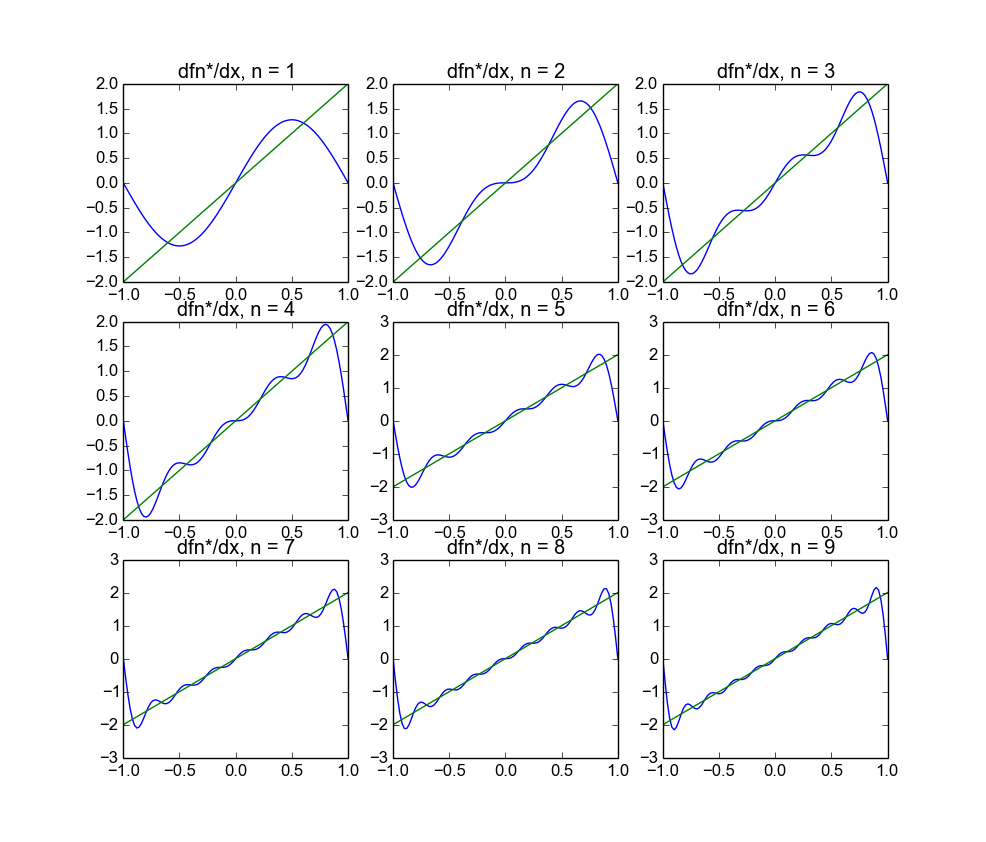
\includegraphics[scale=0.75]{graphsdf.png}
%\clearpage

Now I will show numerically that
\begin{align*}
\dfstardx(\textstyle\frac{2\,n-1}{2\,n+1})-
\displaystyle
\dfdx(\textstyle\frac{2\,n-1}{2\,n+1}) 
\approx 0.36 \quad \mbox{ as $n$ increases}.
\end{align*}

\lstinputlisting{part3.py}
Plotting this difference clearly shows that it tends to 0.36 very quickly.\\
\hspace{-3em}
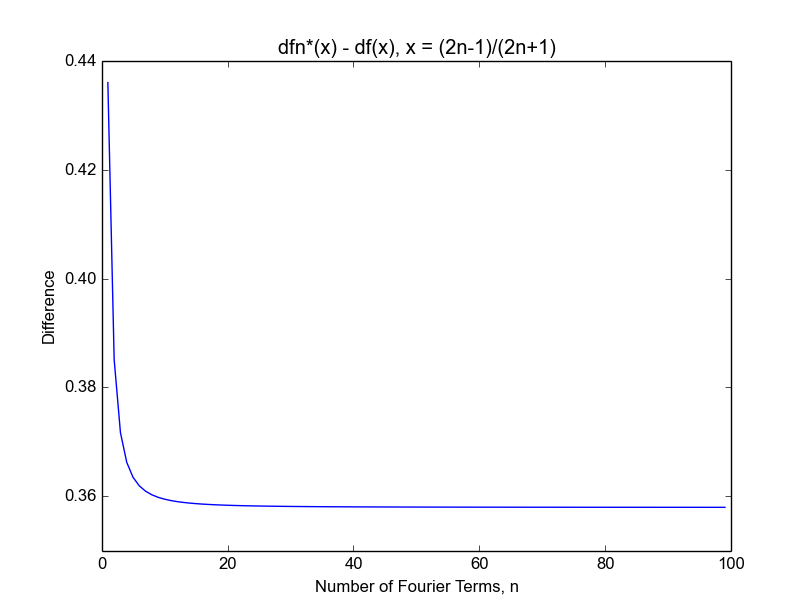
\includegraphics[scale=0.75]{tend036.png}

\clearpage
Finally, on introducing the average
\begin{align*}
s_n(x) = \frac{1}{n+1} \sum_{p=0}^n \dfpstardx (x)\,;
\end{align*}

let's plot $\dfdx(x)$ and $s_n(x)$ for $x \in (-1, 1)$ on one graph for $n = 1 \rightarrow 9$.\\
\hspace{-3em}
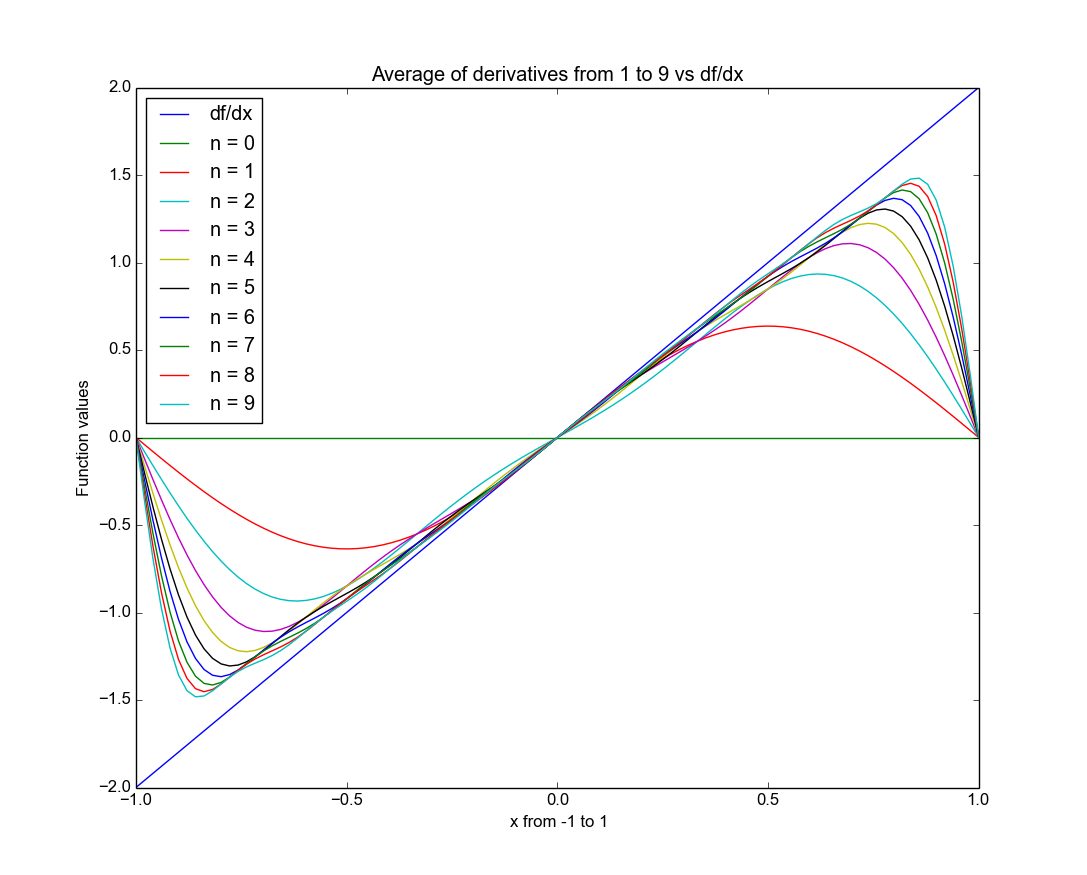
\includegraphics[scale=0.6]{average.png}
\textbf{Observations}\\
As we vary the number of terms in our average, the middle part of our interval has a similar precision. However, the approximation
of the function $f(x) = 2x$ converges to the correct value faster when we include approximations with more terms. This is because
the Fourier Series approximation of a function approaches the true value of the function faster, the more terms it has. We could see
this in the plot of the Fourier Series for the derivative of $f$ in our second plot. When the function has a few terms, it is far from a
good approximation until values of x around $|x| \approx 0.5$. With 9 terms, the approximation is considerably good from around $|x| \approx 0.9$.\\
We generated this using the folowing python code
\lstinputlisting{part4.py}


\end{document}
